\section{Tài nguyên}

\subsection{Bộ dữ liệu}
Báo cáo sử dụng 3 bộ dữ liệu lấy từ dữ liệu chất lượng không khí trên trang web aqicn.org từ 01/03/2019 - 01/06/2024 ở 3 thành phố Hà Nội, Hạ Long và Việt Trì. Bộ dữ liệu bao gồm các thuộc tính cụ thể sau:
\begin{table}[h]
  \centering
  \caption{Mô tả thuộc tính}
  \begin{tabular}{|c|c|}
    \hline
    \textbf{Thuộc tính} & \textbf{Mô tả} \\ \hline
    Ngày & Thời gian (YYYY-MM-DD) \\ \hline
    Pm25 & Bụi mịn có đường kính từ 2.5 đến 10 micron \\ \hline
    Pm10 & Bụi mịn có đường kính nhỏ hơn 2.5 micron \\ \hline
    O3 & Ozon \\ \hline
    NO2 & Đioxit nitơ \\ \hline
    SO2 & Đioxit lưu huỳnh \\ \hline
    CO & Carbon monoxit \\ \hline
  \end{tabular}
\end{table}

\begin{table}[h!]
\centering
\caption{Thống kê mô tả cho Hạ Long, Hà Nội và Việt Trì}
\label{tab:stats}
\begin{tabular}{|c|c|c|c|}
\hline
\textbf{Thống kê} & \textbf{Hạ Long} & \textbf{Hà Nội} & \textbf{Việt Trì} \\
\hline
Count & 1920 & 1920 & 1920 \\
Mean & 40.08 & 63.09 & 42.39 \\
Std Dev & 22.95 & 40.26 & 31.66 \\
Min & 5 & 2 & 1 \\
Q1 & 22 & 31 & 19 \\
Q2 (Median) & 38 & 54.5 & 35 \\
Q3 & 54 & 88 & 59 \\
Max & 163 & 217 & 178 \\
Mode & 5 & 24 & 1 \\
Variance & 527.01 & 1620.88 & 1002.69 \\
Kurtosis & 0.41 & 0.334 & 1.92 \\
Skewness & 0.685 & 0.902 & 1.24 \\
CV & 0.572 & 0.638 & 0.74 \\
\hline
\end{tabular}
\end{table}


% \begin{figure}[H]
%   \centering
%   \begin{minipage}{0.22\textwidth}
%   \centering
%   \end{minipage}
%   \hfill

%   \begin{minipage}{0.23\textwidth}
%       \centering
%       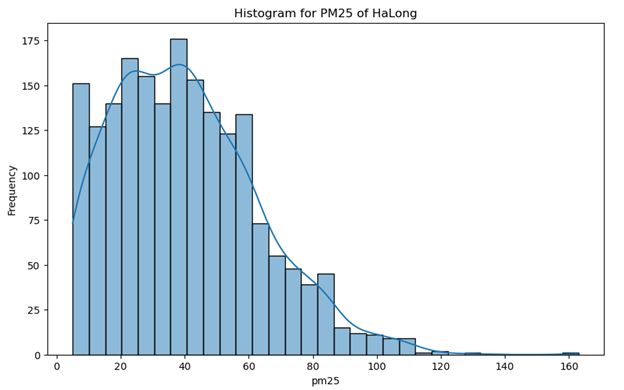
\includegraphics[width=1\textwidth]{img/final/Dataset/histogram.png}
%       \end{minipage}
%       \hfill
%       \begin{minipage}{0.24\textwidth}
%       \centering
%       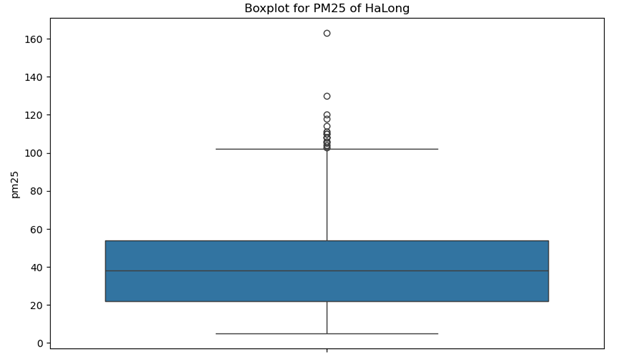
\includegraphics[width=1\textwidth]{img/final/Dataset/boxplot.png}
%       \end{minipage}
  
%   \caption{Biểu đồ histogram và boxplot Hạ Long}
%   \label{fig:Random_Forest}
% \end{figure}

% \begin{figure}[H]
%   \centering
%   \begin{minipage}{0.22\textwidth}
%   \centering
%   \end{minipage}
%   \hfill

%       \begin{minipage}{0.23\textwidth}
%       \centering
%       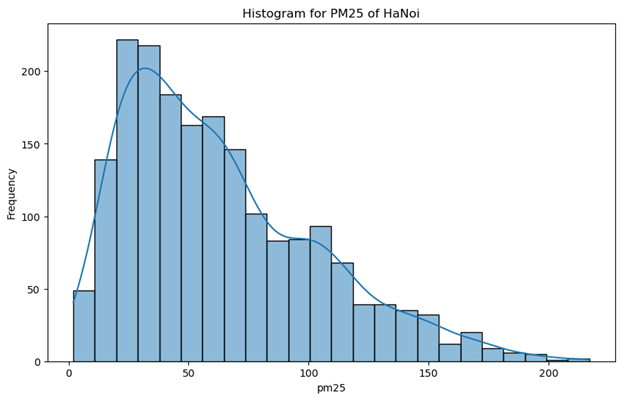
\includegraphics[width=1\textwidth]{img/final/Dataset/histogram_hn.png}
%       \end{minipage}
%       \hfill
%       \begin{minipage}{0.24\textwidth}
%       \centering
%       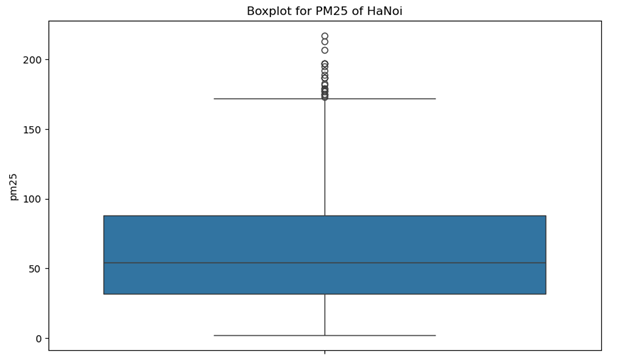
\includegraphics[width=1\textwidth]{img/final/Dataset/boxplot_hn.png}
%       \end{minipage}

%   \caption{Biểu đồ histogram và boxplot Hà Nội}
%   \label{fig:Random_Forest}
% \end{figure}

% \begin{figure}[H]
%   \centering
%   \begin{minipage}{0.22\textwidth}
%   \centering
%   \end{minipage}
%   \hfill

%       \begin{minipage}{0.23\textwidth}
%       \centering
%       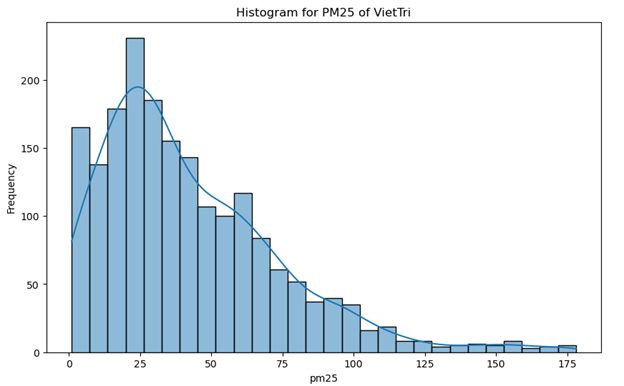
\includegraphics[width=1\textwidth]{img/final/Dataset/histogram_vt.png}
%       \end{minipage}
%       \hfill
%       \begin{minipage}{0.24\textwidth}
%       \centering
%       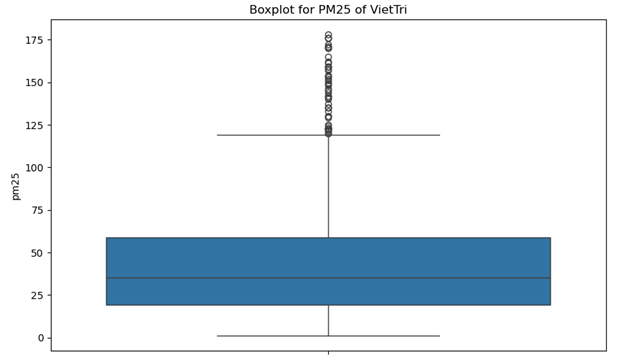
\includegraphics[width=1\textwidth]{img/final/Dataset/boxplot_vt.png}
%       \end{minipage}

%   \caption{Biểu đồ histogram và boxplot Việt Trì}
%   \label{fig:Random_Forest}
% \end{figure}


Hà Nội có giá trị trung bình và mức độ biến động cao nhất trong ba thành phố. Việt Trì có độ nhọn và độ lệch cao nhất, cho thấy dữ liệu phân bố lệch và biến động lớn. Hạ Long có dữ liệu ổn định nhất với giá trị trung bình thấp nhất.


\subsection{Công cụ}
Trong quá trình nghiên cứu và phân tích dữ liệu, Nhóm đã tận dụng một loạt các công cụ phân tích thống kê trong Python để khám phá sâu hơn các mẫu dữ liệu và rút ra những kết luận có ý nghĩa. Các công cụ chính bao gồm: Darts, numpy, pandas, sklearn, matplotlib.pyplot,... Sử dụng các công cụ phân tích thống kê này đã giúp Nhóm em hiểu sâu hơn về dữ liệu và đưa ra dự báo. Chi tiết các kết quả có thể được tìm thấy trong bảng mô tả và biểu đồ đi kèm. 

\subsection{Tỷ lệ phân chia dữ liệu}
Nhóm đã chia tập dữ liệu chuỗi thời gian thành hai phần với các tỷ lệ khác nhau: 70\% huấn luyện và 30\% kiểm tra, 80\% huấn luyện và 20\% kiểm tra, và 90\% huấn luyện và 10\% kiểm tra. Tỷ lệ phổ biến nhất là 70:30, tạo sự cân bằng giữa dữ liệu huấn luyện và kiểm tra. Tỷ lệ 80:20 thích hợp cho các mô hình phức tạp, trong khi 90:10 phù hợp khi xử lý tập dữ liệu lớn và mô hình đơn giản, đảm bảo đủ dữ liệu huấn luyện và kiểm tra. Trong việc đánh giá hiệu suất của các mô hình, Nhóm em sử dụng ba chỉ số là Mean Absolute Error (MAE), Mean Absolute Percentage Error (MAPE), và Root Mean Squared Error (RMSE). Thuật toán có giá trị thấp nhất trong ba chỉ số này sẽ cho thấy mức độ chính xác tốt nhất. Dưới đây là các công thức để tính MAE, MAPE và RMSE.
% \subsection{Đánh giá mô hình}
% Trong việc đánh giá hiệu suất của các mô hình, Nhóm em sử dụng ba chỉ số là Mean Absolute Error (MAE), Mean Absolute Percentage Error (MAPE), và Root Mean Squared Error (RMSE). Thuật toán có giá trị thấp nhất trong ba chỉ số này sẽ cho thấy mức độ chính xác tốt nhất. Dưới đây là các công thức để tính MAE, MAPE và RMSE.
% \subsection*{Với các tham số: }
% \begin{itemize}
%     \item \( n \): Số lượng điểm dữ liệu.
%     \item \( y_i \): Giá trị thực tế.
%     \item \( \hat{y}_i \): Giá trị dự đoán.
% \end{itemize}

% \subsection*{MAE (Lỗi tuyệt đối trung bình):}
% MAE là trung bình của các giá trị tuyệt đối của sai số giữa giá trị dự đoán và giá trị thực tế. Nó đo lường độ lớn của sai số trung bình và không quan tâm đến hướng của sai số. MAE càng nhỏ, mô hình càng chính xác.
% \begin{equation}
% \text{MAE} = \frac{1}{n} \sum_{i=1}^{n} \left| y_i - \hat{y}_i \right|
% \end{equation}

% \subsection*{RMSE (Căn bậc hai của trung bình bình phương sai số):}
% RMSE là căn bậc hai của trung bình của các bình phương của sai số giữa giá trị dự đoán và giá trị thực tế. Nó đo lường độ lớn của sai số trung bình và cung cấp một con số tương đối về mức độ sai lệch giữa dự đoán và giá trị thực tế. RMSE càng nhỏ, mô hình càng chính xác.
% \begin{equation}
% \text{RMSE} = \sqrt{\frac{1}{n} \sum_{i=1}^{n} (y_i - \hat{y}_i)^2}
% \end{equation}

% \subsection*{MAPE (Lỗi phần trăm tuyệt đối trung bình):}
% MAPE là trung bình của tỉ lệ phần trăm của sai số tuyệt đối so với giá trị thực tế. Nó thường được sử dụng để đo lường tỷ lệ phần trăm trung bình của sai số so với giá trị thực tế, cung cấp cái nhìn về mức độ chính xác của mô hình dự đoán. MAPE càng nhỏ, mô hình càng chính xác.
% \begin{equation}
% \text{MAPE} = \frac{1}{n} \sum_{i=1}^{n} \left| \frac{y_i - \hat{y}_i}{y_i} \right| \times 100
% \end{equation}